%\documentclass[english, a4paper]{article}
\documentclass{llncs}
\usepackage{llncsdoc}

\usepackage{float}
\usepackage[pdftex]{graphicx}
\usepackage{caption}
\usepackage[caption=false]{subfig}
\usepackage{url}
\usepackage{siunitx}
\usepackage{graphicx}
\usepackage{pbox} 


\title{Data Mining -- Assignment 1}
\author{Andrew Bedard -- Artagan Malsagov -- Shabaz Sultan}
\begin{document}
\maketitle
\section{Own Dataset Initiative}

\pagebreak
\section{Titanic Survivors\\ \large or: How I learned to Stop Worrying and Love the Data}
%\subsection{Introduction}
%On the 14th of April, 1912 the RMS Titanic hit an iceberg and sank a few hours later. Of the 2207 people on that ship 1501 lost their lives on that night. These tragic events offer the opportunity to study exactly how people behave during such a life-and-death event.\\
%From an economic perspective one can wonder if the model of humans as `homo economicus', that of humans as rational, self-interested actors is the best way to model behaviour of people on that night. An econometric analysis shows that such a `homo economicus' model is overly simplistic because females and children were more likely to survive than physically stronger males. An analysis using said model is still valuable however because people who were closer to their prime age, were of higher social class or had access to more information were more likely to survive\cite{Frey2010}\cite{Frey2011}. \\
%The reason why the deathrate was so high starts with the fact that there were not enough lifeboats. On top of that fewer passengers survived than there was space in lifeboats because of supposed reluctance to leave the ship (e.g. because of disbelief that the ship would actually sink or wives that did not want to be separated from their husbands). The difference in survival between males and females can be explained as a result of policy. The official explanation from the Mersey inquiry to explain the difference in survival rates between classes was that lower-class people were less willing to be parted from their belongings and that their English was poorer making them less able to follow orders from the crew. Statistical analysis based on nationality as a proxy for language ability refutes this second claim and suggest that explanations rejected by the inquiry (layout of the ship disadvantaging lower class people and outright discrimination when letting people on lifeboards) are more likely \cite{Hall1986}.\\
%We can use publicly available data with personal details of Titanic passengers to build our own models to see if we are able to predict survival of a passenger based on things like sex and class.
\subsection{Analysis of the Data}
The data used in this section is provided through the Kaggle website, which host machine learning competitions. The Titanic dataset is intended as one that users can use to practice and get up to speed with machine learning. The data is provided as a list of 891 passengers in a training set and 418 passengers in a test set. Both sets have a number of attributes marked, mentioned in table~\ref{tab:passenger_attributes}.
\begin{table}[H]
\caption{Attributes proved for each passenger in the dataset.}
\label{tab:passenger_attributes}
\centering
\begin{tabular}{ r | l }
  attribute & possible values \\ \hline \hline
  passenger class & 1,2 or 3 (1 is upper class, 3 is lower)  \\
  name & first and last name with title \\
  & (i.e. mr., miss. etc) and possible initials  \\
  sex & male or female \\
  age & number in years \\
  siblings \& spouses & number of siblings and spouses on board \\
  parents \& children & number of parents and children on board \\
  ticket & ticket number \\
  fare & ticket fare \\
  cabin & cabin code (not available for some, multiple for some)\\
  port of embarkation & Cherbourg, Queenstown or Southampton

\end{tabular}
\end{table}
In addition to the attributes mentioned in table~\ref{tab:passenger_attributes} the passengers in the training set also have an attribute denoting if they survived. This allows us to use the training set as the input for a supervised learning model and use said model to create predictions for survival on the test set. 
We can start by gathering some basic statistics on the training set. In the trainingset $38.4\%$ survived. There are 216 first class passengers, 184 second class passengers and 491 third class passengers in the set. The passengers are $64.8\%$ male and $35.2\%$ female.\\
The correlation coefficient between sex and survival is $0.54$, meaning there is a positive correlation between being female and surviving. Next we look at class and survival. There is a positive correlation between being a first class passenger and surviving, with a correlation coefficient of $0.29$. The correlation for second class passengers and survival is $0.09$ and the correlation for third class passengers is $-0.32$.\\
Fare is an alternative marker for socio-economic status. It is correlated with survival at $0.257$. One can wonder how much information the fare attribute adds on top of class. For first class passengers fare further differentiates passengers: there is a correlation with survival of $0.19$. Among second class passengers fare this is $0.10$, for third class passengers this is $0.00$.
\begin{figure}[]
    \centering
   \subfloat[Age distribution of dataset. Mean $29.7$, std.dev. $14.5$, kurtosis $0.18$.]{%
      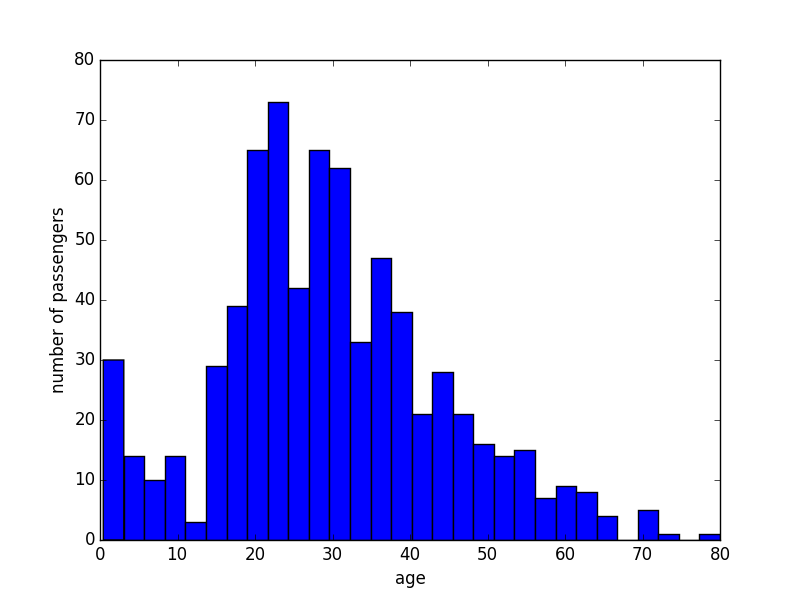
\includegraphics[width=0.30\textwidth]{age_distribution}
    }
    \hfill
   \subfloat[Age distribution of non-survivors. Mean $30.6$, std.dev. $14.2$, kurtosis $0.28$.]{%
      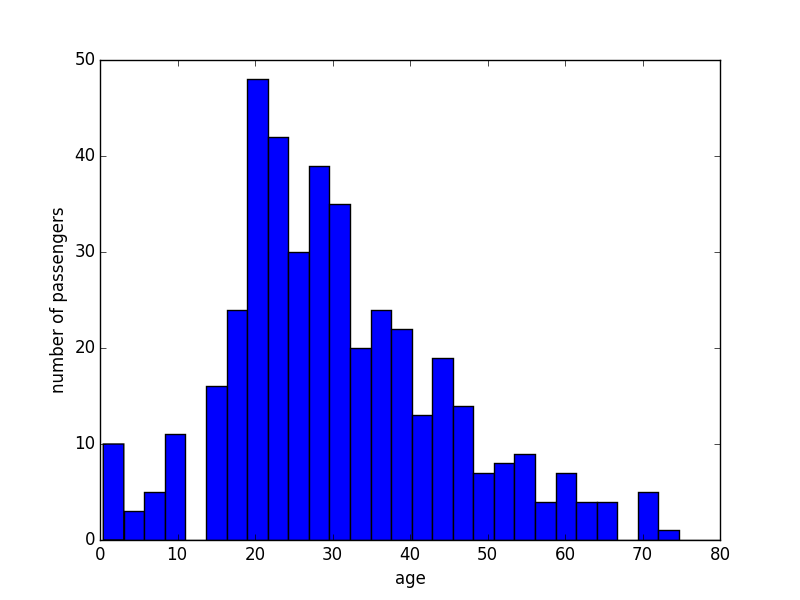
\includegraphics[width=0.30\textwidth]{non_survivor_age_distribution}
    }
    \hfill
    \subfloat[Age distribution of survivors. Mean $28.3$, std.dev. $15.0$, kurtosis $-0.06$.]{%
      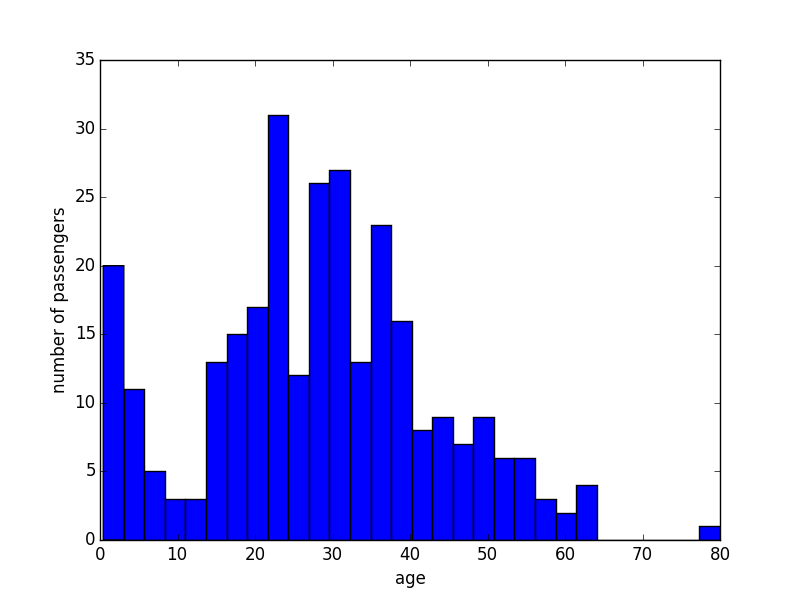
\includegraphics[width=0.30\textwidth]{survivor_age_distribution}
    }
    \caption{Age distributions in the dataset in general and of survivors and non-survivors.}
    \label{fig:age_histogram}.
\end{figure}
\noindent
Only 714 of the 891 passengers in the training set have their age marked. The average age of these 714 passengers is 29.7 years. The distribution of ages is plotted in a histogram in figure~\ref{fig:age_histogram}. Next we look the age distribution between survivors and non-survivors. Judging by the naked eye the two right histograms in figure~\ref{fig:age_histogram} look pretty similar. There is a slight difference in the shape of the two distributions, expressed in the kurtosis.  It seems like age would not have great predictive value for survival, but might be more predictive after the population has been split up based on other criteria first.
%Finally we look at embarkation ports. Based on intuition it seems less likely that this attribute is particularly predictive of survival. Looking at the data however, passengers who embarked from Southampton had a negative correlation with survival at $-0.16$. Passengers from Cherbourg had a positive survival correlation at $0.17$ and those from Queenstown had almost no correlation at $0.00$. One can wonder if these differences can be explained by a difference in e.g. sex and class between passengers from different ports. One way to explore this is building a decision tree with embarkation port, sex and class as attributes and see how far in the tree embarkation port ends up at, which we will try in section~\ref{subsec:titanic_machine_learning_models}.
Using cabin number poses some complication of the attributes handles so far. The dataset is fairly incomplete, only 204 passengers in the training set have a known cabin number. And of those, some of them had multiple cabin numbers, when it was not known exactly which cabin they. Also, the cabin number is a string with a letter and number that needs some pre-processing. If we just look at the correlation of having a known cabin in the dataset and survival the correlation is $0.32$.  The data may be skewed by the fact that a partial list was recovered for the first class cabin allocations\cite{cavelist}, meaning the correlation seen may just be based on class. If we exclude first class passengers we see a smaller correlation of $0.17$ and within the first class group it is $0.15$.\\
The other thing we can do is use the cabin number to figure out a rough position within the ship. The cabin number consist of a letter and a number. The letter denotes the deck. The number denotes the position on the deck. The decks are labeled A to F, with A being closest to the top and F as the bottom deck. There is one passenger with a boat deck cabin, marked with T. One way to use the number is to classify cabins into port and starboard. A lot of tutorials for this dataset report that odd numbered cabins were port side and even numbered cabins were starboard. This is not quite true for every deck (in particular not deck E). With some time exact positions could be constructed from deck layout images to be used, but we will consider this outside of the scope of this report. Instead we'll use the odd/even assignment to port and starboard.\\
If we mark odd as 1 and even as 0 and find the correlation with survival of find a correlation of 0.17 between survival and having a cabin on the port side. If we remove deck E, where we know the even/odd mapping to port and starboard doesn't hold, the correlation becomes a bit stronger at 0.21.
\begin{figure}[H]
    \centering
    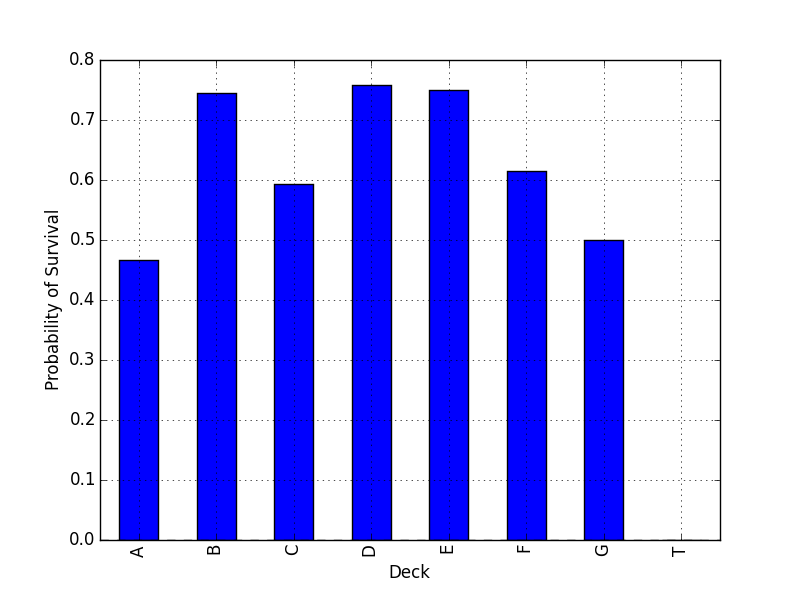
\includegraphics[width=0.4\linewidth]{survival_per_deck}
    \caption{Percentage of survival among passengers on different decks. It should be noted that this is for passengers for whom cabin numbers where known; this is a subset that is more likely to have survived anyway.}
    \label{fig:survival_per_deck}
\end{figure}
\noindent
When we look at the correlation between being on lower deck and surviving, there is small positive correlation of 0.05. This is somewhat surprising because higher class passengers where at higher decks and presumably one has to travel more distance when escaping from a lower deck. However, this dataset is based on the group of passengers where the cabin number was known, which is a biased group anyway that was correlated with higher survival. To gain further insight in the relation between deck and survival, the survival percentage per deck is plotted in figure~\ref{fig:survival_per_deck}.

\subsection{Machine Learning Models}
\label{subsec:titanic_machine_learning_models}

\begin{table}[H]
    \sisetup{round-mode=places}
    \caption{Scores using different classifiers. Scores are found using leave-one-out cross-validation. As a reference accuracy of `always guess non-survival' is 0.61.}
    \label{tab:titanic_model_scores}
    \centering
\resizebox{\linewidth}{!}{%
    \begin{tabular}{ c || S[round-precision=3] | S[round-precision=3] | S[round-precision=3] | S[round-precision=3] | S[round-precision=3]}
        \textbf{fields used} & \textbf{log. regression} & \textbf{SVM} & \textbf{decision tree} & \textbf{naive bayes} & \textbf{random forest} \\ \hline\hline
class and sex & 0.786756453423 & 0.705948372615 & 0.705948372615 & 0.786756453423 & 0.768799102132 \\\hline
class, sex and family size & 0.800224466891 & 0.806958473625 & 0.794612794613 & 0.801346801347 & 0.79797979798 \\\hline
class, sex and known cabin & 0.786756453423 & 0.710437710438 & 0.791245791246 & 0.765432098765 & 0.776655443322 \\\hline
        \pbox{20cm}{class, sex, family size\\ and known cabin} & 0.800224466891 & 0.810325476992 & 0.783389450056 & 0.791245791246 & 0.792368125701 \\\hline
        \pbox{20cm}{class, sex, family size,\\ known cabin and fare} & 0.795735129068 & 0.781144781145 & 0.813692480359 & 0.766554433221 & 0.808080808081 \\\hline
        \pbox{20cm}{class, sex, sibling/spouse,\\ parents/children, known\\cabin and fare} & 0.793490460157 & 0.766554433221 & 0.804713804714 & 0.773288439955 & 0.79797979798 \\ \end{tabular}}
\end{table}
\pagebreak
\section{Research and Theory}
Describing someone else's work is certainly a good way to advance further until you begin to feel your own initiatives coming. Let's try that by starting this section by describing the winning entry of a Kaggle competition.  
\subsection{IJCNN Social Network Challenge}
The Social Network Challenge was hosted by IJCNN and posted on the Kaggle platform in the period of Nov 2010 - Jan 2011. The challenge was to predict edges/connections between nodes/people in an online social network based on an edge dataset obtainted by crawling said network. This dataset was partioned into a training set and a test set, where the test set was expanded by an equal number of fake edges. Predicting then meant the trained algorithm had to classify the $8,960$ test edges as either true or false, after having trained on the $7,237,983$ training edges. As an evalutation measure the area under the ROC-curve was used (AUC), meaning the closer the AUC is to $1$ the better the evaluation of the algorithm. Needless to say user identities of the nodes were obfuscated by assigning random IDs to the nodes in the provided dataset, otherwise a group might cheat its way through.

And the winner was a team going by the name ``IND CCA". Its members wrote their winning approach in an article \cite{6033446} to which the interested reader is referred. The details of their approach are quite intricate, so here's the gist of it. While de-anonymization was forbidden, that is exactly what the winning team did. After finding out the data had been obtained by crawling Flickr, the group decided to crawl Flickr themselves and in so doing managed to de-anonymize $64.7 \%$ of the test edge-set. On the remainder of the test set they used a Random Forest Classifier, training this algorithm on standard link prediction features of both the training and the de-anonymized test set, thus achieving a whopping and winning AUC of $0.981$.

It was this piece of bravado to de-anonymize the test set that made the method stand out. It wasn't blatant cheating, since once the group got a lead in the competition, they contacted the organizers and explained their method, offering to resign all together from the competition. Their method was approved though, and they went on to win the competition. The aim of the slight cheat in their method was of a different kind though, for they wished to raise awareness of the lasting possibility of de-anonymization in machine learning contests and hoped this would provide food for thought on how contest should be run in the future.

\subsection{MSE vs. MAE}
The subject of this part is the use of the two metrics MSE and MAE. A definition of both would be in order: suppose that $\hat{y}$ is a vector of $n$ predicted values and $y$ is the same vector of true values. MSE is measured as:
$$
\frac{1}{n}\sum_{i=1}^{n}(\hat{y_{i}} - y_{i})^{2}
$$  
and MAE measures as:
$$
\frac{1}{n}\sum_{i=1}^{n}|\hat{y_{i}}-y_{i}|
$$
%The two metrics are not expressed in the same unit, for that the square root has to be taken of the MSE, also known as the root mean square error (RMSE): $ \sqrt{\frac{1}{n}\sum_{i=1}^{n}(\hat{y_{i}} - y_{i})^{2}}$. By (mathematical) definition, RMSE is never smaller than the MSE. When the magnitudes of all the differences are equal, RMSE=MAE. 

\noindent The essential difference between the two methods is the MAE assigns the same weights to all deviations when averaging over the sample, whereas the MSE weighs a deviation by that very same deviation, assigning high weights to high deviations and thus penalizing high errors. This mechanism of MSE to overweigh tail events prevents large errors but the trade-off is that it also may commit more smaller errors. Imagine the errors are smaller than $1$ in absolute values, in that case MSE will be smaller than MAE. It commits less of these smaller errors due to equal weighing.

On the other hand, if large errors are the main concern, than MSE is the tool of the trade. Also, the squared difference is much more ``well-behaved" than the absolute difference. It is continuously differentiable, which is handy for minimization. It equals the sample variance (biased) when for all $i$ the sample mean of the $y_{i}$s is taken as a predictor. Finally, it also ties in with the Euclidean distance, which makes it useful for proving limit theorems.

Suppose we are dealing with a classification problem and the vector of true values $y=[y_{1},\dots,y_{n}]^{T}$ is binary. Then the errors are either $0$ or $1$ in absolute value and likewise when squared, i.e. $(\hat{y_{i}} - y_{i})^{2}=|\hat{y_{i}}-y_{i}|$ for all $i$. Averaging over all $n$ errors gives then the same value for the MSE and MAE.

\subsubsection{Examples}
Let's try doing a real example; for that we use a dataset from \cite{Longl}, also called the Longley dataset; it was downloaded from source \cite{WinNT}. This data set consists of highly collinear macro-economic variables. Each instance in the data set corresponds to a year in the period of 1947-1962, where GNP, GNP deflator, unemployed population, employed population, armed forces population, entire population, year were all recorded as variables.

%\begin{table}[H]
%\caption{Variables of Longley dataset}
%\label{tab:passenger_attributes}
%\centering
%\begin{tabular}{ r | l }
%  Variables & units\\ \hline \hline
%  GNP deflator & percentage \\ 
%  GNP & reals   \\
%  Unemployed & thousands \\
%  Armed forces & thousands\\
%  Population & thousands\\
%  Year &  years \\
%  Employed & thousands
%\end{tabular}
%\end{table}

Before we discussed the fact that MSE shrugs off the occurrence of smaller errors, while MAD takes them into account. This dataset shall aid us in illustrating the point. The variables are highly collinear and can thus explain each other well in a regression, providing small errors. Let's use ``Employed" as the dependent variable of our regression, and start out modestly by regressing it on one explanatory variable ``GNP" and a constant. So a very general linear regression: $\displaystyle y = \beta_{0} + \beta_{1}x$ where $x$ obviously stands for GNP. Indeed, one would expect the national product and employment to be related, in a positive way. But there might also be a saturation, so the positive effect of GNP on employment might reach a limit. This can be captured by adding a quadratic term to the regression for GNP: $\displaystyle y = \beta_{0} + \beta_{1}x +\beta_{2}x^{2}$. The MSE and MAE of the two regressions programmed in Python are summarized below.

\begin{table}[H]
    \centering
    \begin{tabular}{l | c | c}
        & MSE & MAE\\ \hline
        simple regression & 0.37& 0.51 \\
        quadratic regression & 0.35 & 0.49
    \end{tabular}
    \caption{MSE and MAE of the simple linear and quadratic regression}
    \label{table:MSE_vs_MAE}
\end{table}
\noindent Note the MSE is smaller than the MAE in both cases. The potential danger here is that the model seems better under the MSE than under the MAE. If small errors aren't of concern in the case at hand, something you could argue for predicting employment, then both metrics seem reliable. However, situations requiring preciser prediction can be imagined, and the difference does matter. In the end it all depends on the given context, but being aware of these issues between the two metrics is crucial.

\subsection{SMS dataset: text mining Ham and Spam}
The data in the SMS dataset consists of text messages labelled as either spam or ham. The aim is to model this data and be able to predict whether a message is spam or ham. A way to model this is with the            
\bibliographystyle{plain}
\bibliography{report}
\end{document}
